\documentclass[12 pt, a4paper]{article}
\usepackage[norsk]{babel}  								% For norsk oppsett
\usepackage[utf8]{inputenc}
\usepackage{amsmath}
\usepackage{amssymb}
\usepackage{graphicx}
\usepackage{subcaption}
\usepackage{hyperref}
\usepackage{fancyhdr}
\usepackage{enumerate}
\usepackage{float}
\usepackage{tikz}
\usepackage{circuitikz}
\usepackage{tabularx}
\usepackage{physics}
%\usepackage[includeheadfoot, margin =1cm]{geometry}
%\usepackage{python}
\usepackage[version=3]{mhchem}
\usepackage{siunitx}
\usepackage{todonotes}
\usepackage{xcolor}
\usepackage{lastpage}
\usepackage{listings}
\renewcommand{\exp}[1]{\mathrm{e}^{#1}}

\lstset{basicstyle=\ttfamily,
  showstringspaces=false,
  commentstyle=\color{red},
  keywordstyle=\color{blue}
}

\usepackage[bottom]{footmisc}
\renewcommand\footnoterule{\rule{\linewidth}{0.5pt}}

\setlength{\parindent}{0cm}

\author{Mikael B. Kiste}
\title{STK1000 - oblig 1}

\begin{document}
\maketitle
\newpage

%\pagestyle{fancy}
%\fancyhf{}
%\rhead{STK1000 - Oblig 1}
%\lhead{Erik Skaar}
%\fancyfoot[CE,LO]{\leftmark}
%\fancyfoot[LE,RO]{Page \number\value{page} of \pageref{LastPage}}

%\renewcommand{\headrulewidth}{2pt}
%\renewcommand{\footrulewidth}{1pt}

\section{}%1

\subsection*{a}
Her er et histogram av BMR verdiene til sebrafinkene. Histogrammet ser normalfordelt ut, med en god del sebrafinker som har en BMR verdi nær gjennomsnittet og et kraftig avtagende antall finker jo lenger man går vekk fra gjennomsnittet. 
\begin{figure}[H]
        \centering
        \includegraphics[width=0.9\linewidth]{zebrafish.pdf}
        \caption{Histogram av BMR-verdiene til 150 zebrafisker}
        \label{fig:histogram}
\end{figure}


\subsection*{b}

Ved å bruke kommandoen \texttt{mean} i R får jeg gjennomsnitt og \texttt{median} gir meg median.
\begin{align*}
    \bar{x} = 0.8485003\mathrm{mL}\frac{o_2}{\mathrm{m}}\\
    \mathrm{mean} = 0.8397846\mathrm{mL}\frac{o_2}{\mathrm{m}}
\end{align*}
Gjennomsnittet tar summen av måleverdien til alle datapunktene før det deler på antall datapunkter mens median er verdien på det midterste elementet i en ordnet (numerisk økende) liste av datapunktene.

\subsection*{c}

Ved å bruke kommandoen \texttt{IQR} i R får jeg inter-kvartil og \texttt{sd} gir meg standardavvik.
\begin{align*}
    \mathrm{IQR} = 0.1517731\mathrm{mL}\frac{o_2}{\mathrm{m}}\\
    \sigma = 0.1134001\mathrm{mL}\frac{o_2}{\mathrm{m}}
\end{align*}

\subsection*{d}

Ved å bruke kommandoene \texttt{qqnorm()} i R får jeg inter-kvartil og \texttt{sd()} gir meg standardavvik.

\begin{figure}[H]
        \centering
        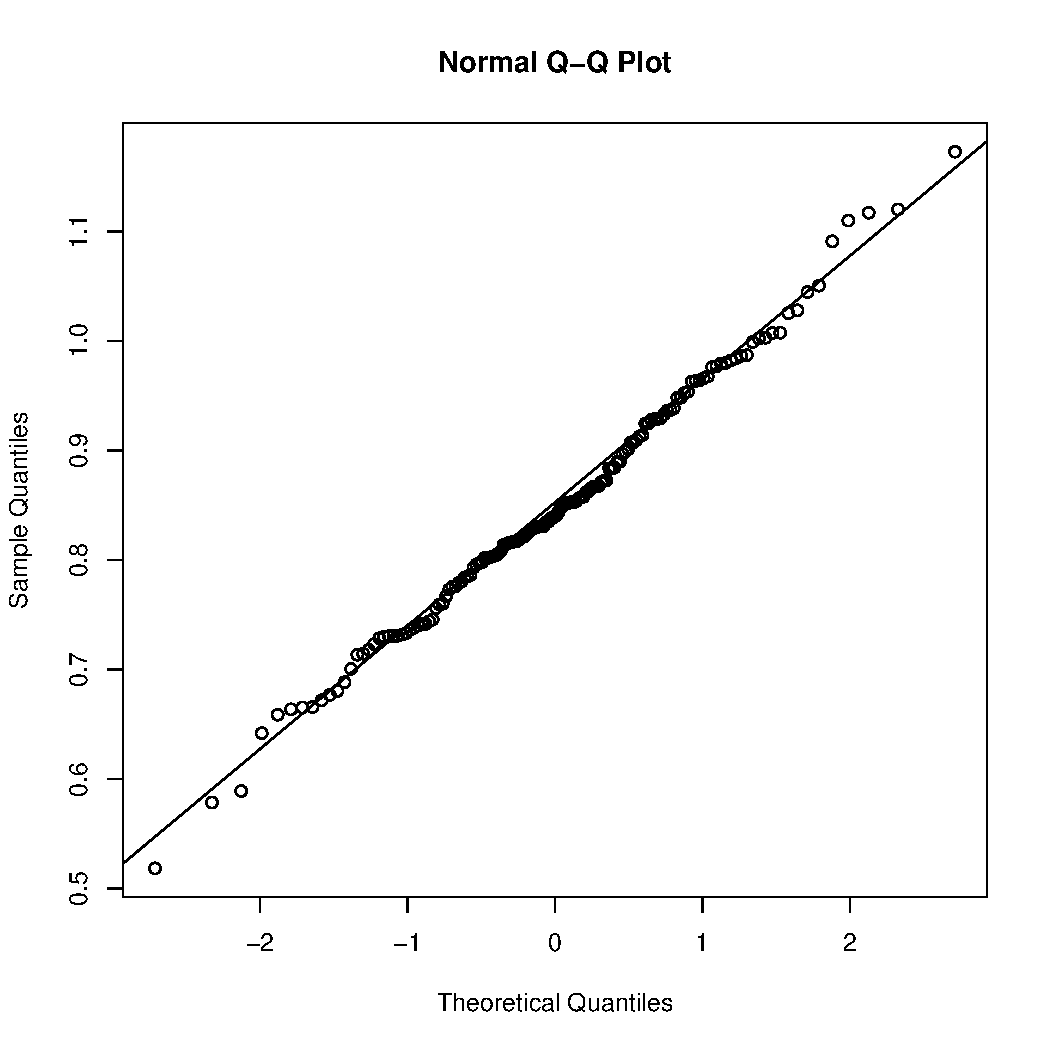
\includegraphics[width=0.9\linewidth]{Rplots.pdf}
        \caption{Figuren viser målte verdier mot standardavviket vi fikk tidligere i oppgaven}
        \label{fig:QQ}
\end{figure}
Plottet indikerer hvordan de målte verdiene har fordelt seg i forhold til standardavviket. Igjen ser man at de fleste datapunktene legger seg rundt gjennomsnittet, men i tillegg får man et inntrykk av hvordan målverdiene avviker fra den teoretiske perfekte normalfordelingen (over eller under den lineære funksjonen). Man kan se at dataen passer ganske bra til en normalfordeling.

\subsection*{e}

Standardiserte verdien til BMR:
Den standardiserte verdien, eller 'z-score', antyder hvor mange standardavvik en målverdi er fra gjennomsnittet. Altså

\begin{align*}
    z = \frac{x - \mu}{\sigma}
\end{align*}

For BMR = 0.8 mL O$_2$/min gir det:
\begin{align*}
    z = \frac{x - \mu}{\sigma} = \frac{0.8 - 0.8485003}{0.1134001} \approx -0.43
\end{align*}
Målverdien på $0.8\mathrm{mL}\frac{o_2}{\mathrm{m}}$ er $-0.43$ standardavvik unna gjennomsnittet.

\subsection*{f}

Ved å bruke kommandoen \texttt{pnorm()} i R får jeg prosentilen til en BMR på $0.6$
\begin{align*}
    p(x<0.6) = 0.01421294
\end{align*}

\subsection*{g}
På samme måte som i forrige oppgave bruker jeg \texttt{pnorm()}, men denne gangen tar jeg én og trekker i fra sannsynligheten for å finne ut sannsynligheten for at en fink har en BMR som er OVER dette.)
\begin{align*}
    p(x>1.0) = 0.09077876
\end{align*}

\pagebreak
\section{}


\subsection*{a}
Kvantitative variabler er variabler som har en konkret tallverdi. Dette tillater at flere nyttige numeriske operasjoner kan utføres på et datasett av kvantitative variabler. Konsentrasjon av kortisol og testosteron er også kvantitative\\
Kvalitative variabler derimot kan være mer abstrakte. Som for eksempel øyenfarge.\\
Kategoriske variabler er alltid medlemmer av et gitt sett av mulige verdier. Innen vitenskap er det for eksempel fortsatt slik at nesten utelukkende alle dyr kun kan ha ett av to kjønn: han (maskulin) eller hun (feminin). Kjønn er altså et eksempel på en kategorisk variabel. I dette tilfellet er også populasjon kategorisk når den kun deler populasjonen inn i ulv som er hardt jaktet eller ikke. Legg merke til at denne også er en kvalitativ variabel. Kategoriske variabler kan være enten kvalitative eller kvantitative.

\subsection*{b}

Ved å bruke kommandoene \texttt{pie(table(variabel))} i R får jeg et kakediagram over de kategoriske variablene. 

\begin{figure}[H]
        \centering
        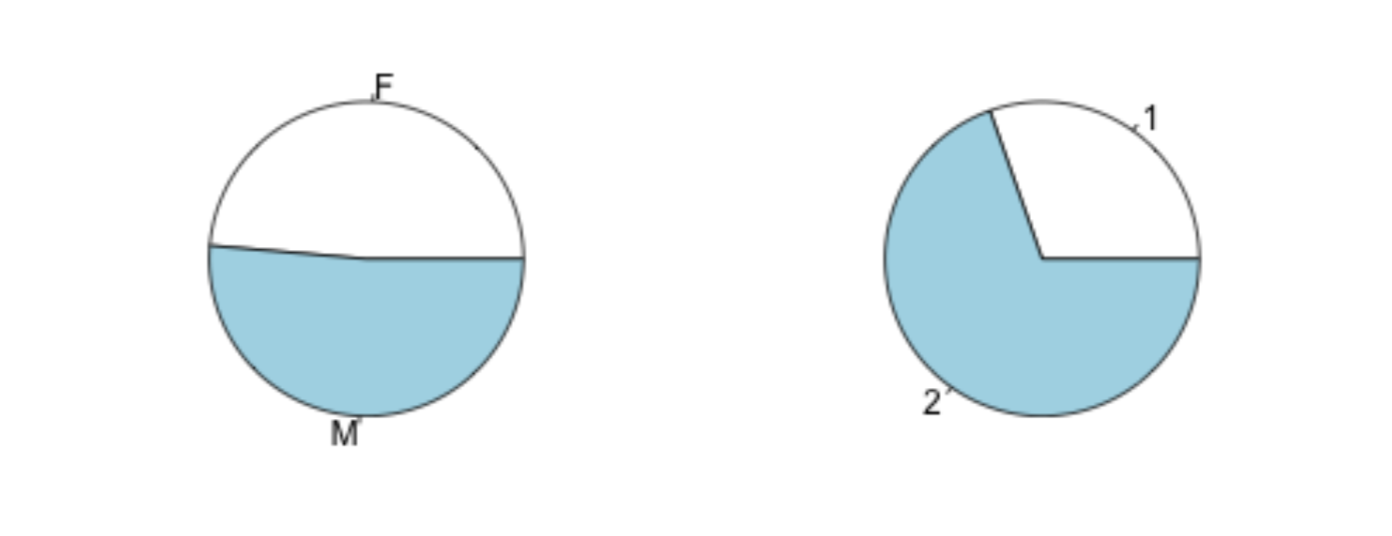
\includegraphics[width=0.7\linewidth]{wolf_sex.png}
        \caption{kjønnsfordelingen blandt ulvepopulasjonen er svært jevnt fordelt, hvilket nesten alltid er tilfellet pga naturlig seleksjon. Omtrent to tredeler er tungt jaktet}
        \label{fig:sex_population}
\end{figure}

\subsection*{c}

Denne oppgaven løser jeg ved å bruke kommandoene \texttt{wolf.lett <- wolf[wolf[,"population"]==1,]} og \texttt{wolf.tungt <- wolf[wolf[,"population"]==2,]}, slik jeg ble fortalt i oppgaven.

\subsection*{d}
Her bruker jeg de følgende kommandoene:

\begin{itemize}
    \item \texttt{par(mfrow=c(2,2))}
    \item \texttt{hist(wolf.lett)}
    \item \texttt{boxplot(wolf.lett)}
    \item \texttt{hist(wolf.tungt)}
    \item \texttt{boxplot(wolf.tungt)}
\end{itemize}
Hvordan disse fungerer er kommentert i koden
\begin{figure}[H]
        \centering
        \includegraphics[width=0.9\linewidth]{wolf_sammenlign.pdf}
        \caption{Her er histogram og boxplott av kortisolkonsentrasjonen til ulv som har blitt lett jaktet (øverst) og tungt jaktet (nederst)}
        \label{fig:sammenlign}
\end{figure}
Man kan se at ulv som har blitt tungt jaktet har høyere konsentrasjon av kortisol.

\subsection*{e}

I begge tilfeller er medianen mindre enn gjennomsnittet. Dette antydes også gjennom histogrammene

\begin{center}
\label{tab:mean_median_standard}
\captionof{table}{Tabell over gjennomsnitt, median og standardavvik}
\begin{tabularx}{\textwidth}{c X c X c X c }
    \hline
    \hline
         && Mean && Median && Standard deviation \\
    \hline
    \\
        Lett    &&     15.56222      &&      14.24      &&     7.298785       \\
        Tungt   &&     17.07495      &&      16.32      &&      5.543389       \\
    \hline
\end{tabularx}
\end{center}


\subsection*{f}
For normalfordelte datasett holder det å oppgi gjennomsnitt og standardavvik for å tilstrekkelig beskrive fordelingen. I andre tilfeller trenger man mer informasjon og da kan det være nyttig å bruke en femtallsoppsummering som i tillegg gir minimumverdi, maximumverdi og kvartiler.
For å svare på spørsmålet må vi altså se på populasjon og avgjøre om de er normalfordelt eller ikke

\subsection*{g}

\begin{figure}[H]
    \centering
    \begin{subfigure}{0.5\textwidth}
        \centering
        \includegraphics[width=\linewidth]{LETT.pdf}
        \caption{Lett jaktet ulv}
    \end{subfigure}%
    ~
    \begin{subfigure}{0.5\textwidth}
        \centering
        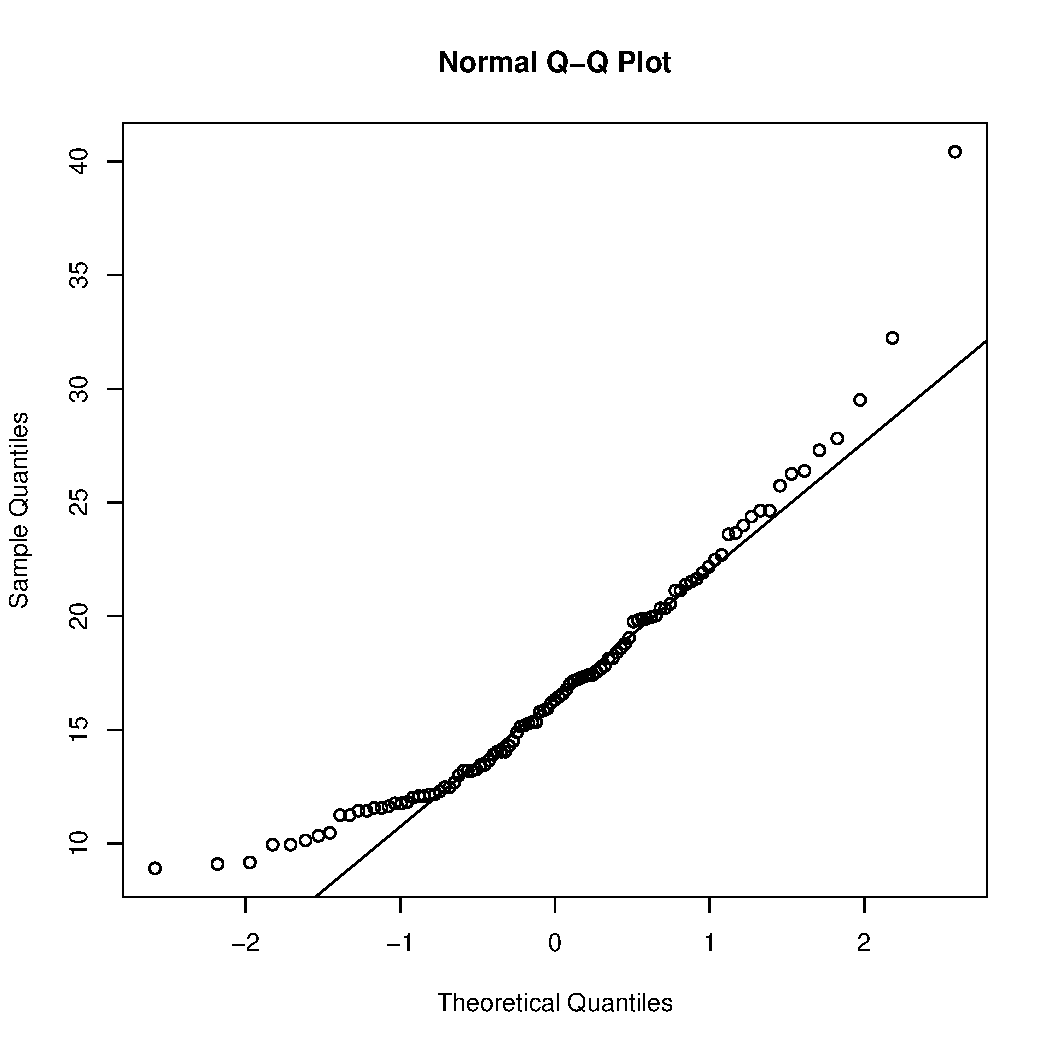
\includegraphics[width=\linewidth]{TUNGT.pdf}
        \caption{Tungt jaktet ulv}
    \end{subfigure}
    \caption{QQ plot over kortisolnivå for populasjonene}
    \label{fig:2G}
\end{figure}

Fra figur \ref{fig:2G} ser det ut til at tungt jaktet ulv er normalfordelt mens lett jaktet ulv ikke er det. Altså kan en bruke gjennomsnitt og standardavvik for å tilstrekkelig beskrive den tungt jaktede populasjonen mens for den lett jaktede populasjonen bør man bruke femtallsoppsummering.

\pagebreak
\section{}

\subsection*{a}

I denne oppgaven bruker jeg kommandoen \texttt{summary()}

150 kvinner og 73 menn deltok i forsøket

\begin{center}
\label{tab:summary}
\captionof{table}{Fem-punkts oppsummering av de fire variablene}
\begin{tabularx}{\textwidth}{c X c X c X c X c X c }
    \hline
    \hline
         && min && $Q_1$ && $\mu$ && $Q_3$ && max \\
    \hline
    kroppslengde    && 152.0 && 166.0 && 172.3 && 178.0 && 196.0 \\
    fot.navle       &&  87.0 && 101.0 && 104.8 && 109.0 && 125.0 \\
    navle.isse      && 52.00 && 65.00 && 67.34 && 70.00 && 81.00 \\
    favn            && 146.0 && 165.0 && 172.4 && 180.0 && 202.0 \\

    \hline
\end{tabularx}
\end{center}

\subsection*{b}
I denne oppgaven bruker jeg kommandoen \texttt{plot()} i for å lage et spredningsplot. 

\begin{figure}[H]
        \centering
        \includegraphics[width=0.9\linewidth]{3B.pdf}
        \caption{Her er et plot av kroppslengde som funksjon av navlehøyde}
        \label{fig:3B}
\end{figure}
Man kan se at det er høy korrelasjon mellom kroppslengde og navlehøyde

\subsection*{c}
I denne oppgaven bruker jeg kommandoen \texttt{cor()} for å få korrelasjonen. En korrelasjon på 0.9140397 antyder igjen at det er en god sammenheng mellom kroppslengde og navlehøyde.

\subsection*{d}
Her er koden justert litt i forhold til det som ble oppgitt i oppgaveteksten

\begin{figure}[H]
        \centering
        \includegraphics[width=0.9\linewidth]{3D.pdf}
        \caption{Lineær regresjon utført på kroppslengde som funksjon av navlehøyde}
        \label{fig:3D}
\end{figure}


\subsection*{e}

\begin{center}
\label{tab:e}
\captionof{table}{Koeffisienter for modellen}
\begin{tabularx}{\textwidth}{c X c X c }
    \hline
    \hline
        Koeffisienter && a && b\\
    \hline
                    && 38.897 && 1.273\\
    \hline
\end{tabularx}
\end{center}

I denne oppgaven brukte jeg \texttt{print(fit)} for å få ut koeffisientene til den lineære tilpasningen av funksjonen. Det ser ut til at en økning på navlehøyde med én cm vil, i gjennomsnitt, føre til en høydeøkning på 1.273 cm. Stigningstallet er mer enn én, men fortsatt en konstant verdi (pga. den lineære tilpasningen).

\subsection*{f}
Her er det rett og slett å bare ta produktet med det lineære forholdet vi fant i forrige oppgave mens man husker på å inkludere verdien hvor den lineære funksjonen skjærer y aksen. Altså funksjonsverdien til den lineære funksjonen med riktige koeffisienter a og b

\begin{align*}
    f(121)= a + bx = 192.93
\end{align*}

\subsection*{g}

\begin{center}
\label{tab:summary2}
\captionof{table}{...}
\begin{tabularx}{\textwidth}{c X c X c X c X c X c }
    \hline
    \hline
         && min && $Q_1$ && $\mu$ && $Q_3$ && max \\
    \hline
    kroppslengde    && 152.0 && 166.0 && 172.3 && 178.0 && 196.0 \\
    fot.navle       &&  87.0 && 101.0 && 104.8 && 109.0 && 125.0 \\
    navle.isse      && 52.00 && 65.00 && 67.34 && 70.00 && 81.00 \\
    favn            && 146.0 && 165.0 && 172.4 && 180.0 && 202.0 \\

    \hline
\end{tabularx}
\end{center}
Fra tabellen kan man se at det er en viss andel av variasjonen i kroppslengde som forklares av navlehøyde. Dette samsvarer godt med det vi fant ut i forrige oppgave. 

\subsection*{h}

\begin{figure}[H]
        \centering
        \includegraphics[width=0.7\linewidth]{3H.pdf}
        \caption{Plott over residualene av navlehøyde i forhold til den lineære modellen}
        \label{fig:3H}
\end{figure}

Det vil alltid være noen uteligger for enhver rimelig regresjonstilpasning. Her ser det ut til at residualene er nogelunde jevnt fordelt, hvilket kan være et godt tegn. Mange datapunkter som ligger enten over eller under modellen vil aldri være tilfellet ettersom regresjonstilpasningen ville justert for dette. Det man kan prøve å se etter, derimot, er om det ser ut til at residualene følger en systematisk trend som ikke er jevnt fordelt. For eksempel, hvis man prøver en lineær tilpasning på et andregradspolynom, ville man kanskje sett at datapunktene i midten ligger under det modellen skulle tilsi mens datapunktene lenger ut ligger over. Men, som sagt, dette ser ikke ut til å være tilfellet her.

\pagebreak

\section*{Appendix}
\subsection{Oppgave 1}
\lstinputlisting[language=R]{1.R}
\newpage
\subsection{Oppgave 2}
\lstinputlisting[language=R]{2.R}
\newpage
\subsection{Oppgave 3}
\lstinputlisting[language=R]{3.R}

\end{document}